\section{Introduction}
\subsection{Metric Spaces}

\begin{definition}[Metric Space]
    A set $X$ is a \emph{metric space} with distance $d$ if 
    \begin{enumerate}
        \item (symmetric) $d(x, y) = d(y, x) \geq 0$
        \item $d(x, y) = 0 \iff x = y$
        \item (triangle inequality) $d(x,y) + d(y, z) \geq d(x, z)$
    \end{enumerate}
\end{definition}

\begin{remark}
    If 1., 3. are satisfied but not 2., $d$ can be called a "pseudo-distance".
\end{remark}

\begin{definition}[Normed Space]
    Let $X$ be a vector space over $\mathbb{R}$. The norm on $X$, denoted $||x|| \in \mathbb{R}$, is a function that satisfies 
    \begin{enumerate}
        \item $\norm{x} \geq 0$
        \item $||x|| = 0 \iff x = 0$
        \item $||c \cdot x|| = \abs{c} \cdot \norm{x}$
        \item $||x+y|| \leq ||x|| + ||y||$
    \end{enumerate}
    If $X$ is a normed vector space over $\mathbb{R}$, we can define a distance $d$ on $X$ by $d(x,y) = \norm{x - y}$.
\end{definition}

\begin{proposition}
    If $X$ is a normed vector space over $\mathbb{R}$, a distance $d$ on $X$ by $d(x,y) = \norm{x - y}$ makes $(X, d)$ a metric space.
\end{proposition}

\begin{proof}
    \begin{enumerate}
        \item $d(x,y) = \norm{x - y} \geq 0$
        \item $d(x, y) = 0 \iff \norm{x - y} = 0 \iff x - y = 0 \iff x = y$
        \item $d(x, y) + d(y, z) = \norm{x - y} + \norm{y - z} \geq \norm{(x - y) + (y-z)} = \norm{x - z} := d(x, z)$
    \end{enumerate}
\end{proof}

\begin{example}[$L^p$ distance in $\mathbb{R}^n$]
    Let $\overline{x} \in \mathbb{R}^n, x = (x_1, x_2, \dots, x_n)$. The $L^p$ norm is defined \[
    \norm{x}_p := (\abs{x_1}^p + \abs{x_2}^p + \cdots + \abs{x_n}^p)^{\frac{1}{p}}.    
    \]
    In the case $p = 2, n = 2$, we simply have the standard Euclidean distance over $\mathbb{R}^2$.

    \underline{Unit Balls:} consider when $\norm{x}_p \leq 1$, over $\mathbb{R}^2$.
    \begin{itemize}
        \item $p = 1:$ $\abs{x_1} + \abs{x_2} \leq 1$; this forms a "diamond ball" in the plane.
        \item $p = 2:$ $\sqrt{\abs{x_1}^{2}+\abs{x_2}^2} \leq 1$; this forms a circle of radius 1. Clearly, this surrounds a larger area than in $p =2$.
        % TODO
    \end{itemize}
    A natural question that follows is what happens as $p \to \infty$? Assuming $\abs{x_1} \geq \abs{x_2}$:
    \begin{align*}
        \norm{x}_p = \left(\abs{x_1}^p + \abs{x_2}^p\right)^{\frac{1}{p}}\\
        = \left[\abs{x_1}^p\left(1 + \abs{\frac{x_2}{x_1}}^p\right)\right]^{\frac{1}{p}}\\
        = \abs{x_1}\left(1 + \abs{\frac{x_2}{x_1}}^p\right)^{\frac{1}{p}}
    \end{align*}
    If $\abs{x_1} > \abs{x_2}$, this goes to $\abs{x_1}$. If they are instead equal, then $\norm{x}_p = \abs{x_1}\cdot 2^{\frac{1}{p}} \to \abs{x_1} \cdot 1$ as well. Hence, $\lim_{p \to \infty} \norm{x}_p = \max\{\abs{x_1}, \abs{x_2}\}$. Thus, the unit ball will approach $\max \{\abs{x_1}, \abs{x_2}\} \leq 1$, that is, the unit square.
\end{example}
\begin{figure*}[!ht]
    \centering
    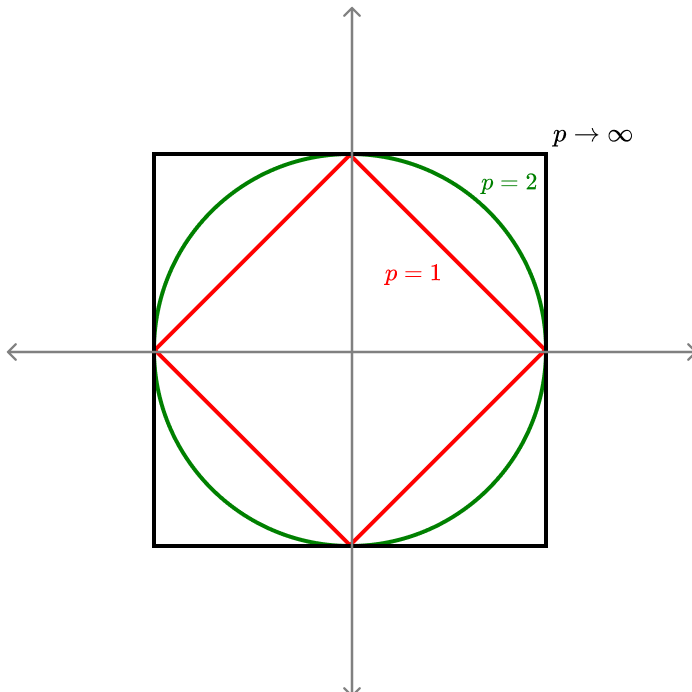
\includegraphics[width=0.5\textwidth]{misc/unitballs.png}
    \caption{Regions of $\mathbb{R}^2$ where $\norm{x}_p \leq 1$ for various values of $p$.}
\end{figure*}
\begin{proposition}
    Let $x \in \mathbb{R}^n$. Then, $\norm{x}_p \to \max \{\abs{x_1}, \dots, \abs{x_n}\}$ as $p \to \infty$.
\end{proposition}

\begin{remark}
    This is an extension of the previous example to arbitrary real space.
\end{remark}

\begin{proof}
    % TODO
\end{proof}

\begin{definition}[Convex Set]
    Let $X$ be a normed space, and take $x, y \in X$. The line segment from $x$ to $y$ is the set \[
    \{t \cdot x  + (1 - t)\cdot y: 0 \leq t \leq 1\} .
    \]
    Let $A \subseteq X$. $A$ is \emph{convex} $\iff \forall x,y \in A$, we have that $$(t \cdot x + (1- t)\cdot y) \in A \forall 0 \leq t \leq 1.$$
\end{definition}

\begin{figure*}[!ht]
    \centering
    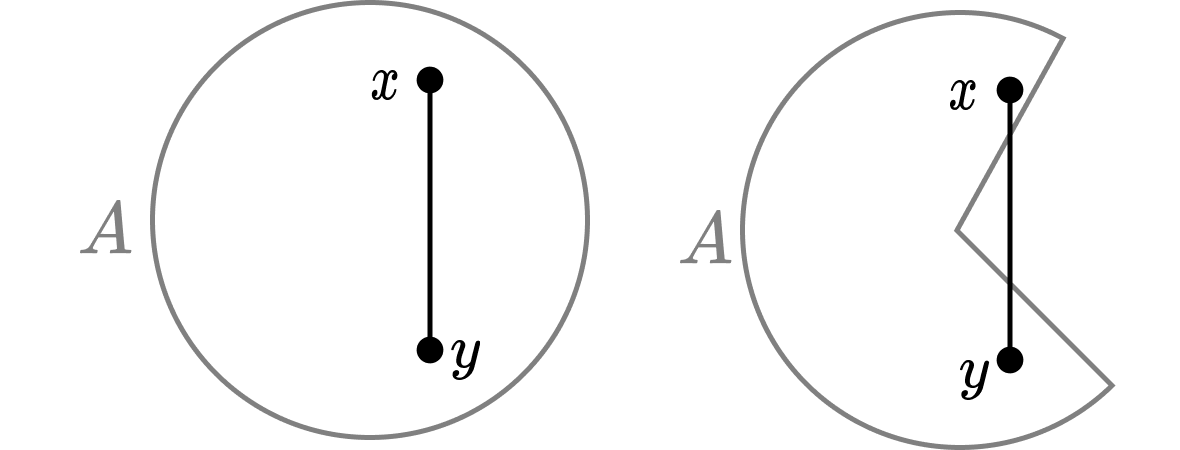
\includegraphics[width=0.5\textwidth]{misc/convex.png}
    \caption{Convex (left) versus not convex (right) sets.}
\end{figure*}

\begin{remark}
    Think of this as saying "a set is convex iff every point on a line segment connected any two points is in the set".
\end{remark}

\begin{definition}[$\ell_p$]
    The space $\ell_p$ of sequences is defined as \[
    \{x = (x_1, x_2, \dots, x_n, \dots) : \sum_{n=1}^{\infty} \abs{x_n}^p < + \infty\} \quad \ast.
    \]
    Then, $\ast$ defines the $\ell^p$ norm on the space of sequences; that is, $\norm{x}_p := \left(\sum_{n = 1}^\infty \abs{x_n}^p\right)^{\frac{1}{p}}$.
\end{definition}

\begin{example}[$\ell_p$, $x_n = \frac{1}{n}$].
   Let $x_n = \frac{1}{n}$. For which $p$ is $x \in \ell_p$? We have, raising the norm to the power of $p$ for ease:
   \begin{align*}
    \norm{x}_p^p = \abs{x_1}^p + \abs{x_2}^p + \cdots + \abs{x_n}^p + \cdots\\
    = 1^p + \left(\frac{1}{2}\right)^p + \cdots < \infty \iff p > 1.
   \end{align*}
   In the case that $p = 1$, this becomes a harmonic sum, which diverges.
\end{example}

\begin{example}[$L^p$ space of functions]
    Let $f(x)$ be a continuous function. We define the norm of $f$ over an interval $[a, b]$
    $$
    \norm{f}_p = \left[\int_{a}^{b}\abs{f(x)}^p dx \right]^{\frac{1}{p}}.
    $$
\end{example}

\begin{remark}
    Triangle inequality for $\norm{x}_p$ or $\norm{f}_p$ is called Minkowski inequality; $\norm{x}_p + \norm{y}_p \geq \norm{x + y}_p$. This will be discussed further.
\end{remark}

\begin{example}[Distances between sets in $\mathbb{R}^2$]
    Let $A, B$ be bounded, closed, "nice" sets in $\mathbb{R}^2$. We define \[
        d(A, B) := \text{Area}(A \triangle B),
        \]
        where $$A \triangle B : (A \setminus B) \cup (B \setminus A) = (A \cup B) \setminus (A \cap B).$$ It can be shown that this is a "valid" distance.
        % TODO
\end{example}

\begin{remark}
    $\triangle$ denotes the "symmetric difference" of two sets.
\end{remark}

% \begin{example}[Hausdorff Distance]
%     %
% \end{example}

\begin{example}[$p$-adic distance]
    Let $p$ be a prime number. Let $x = \frac{a}{b} \in \mathbb{Q}$, and write $x = p^k\cdot \left(\frac{c}{d}\right),$ where $c, d$ are not divisible by $p$. Then, the $p$-adic norm is defined $\norm{x}_p := p^{-k}$. It can be shown that this is a norm. 

    Suppose $p = 2$, $x = 28 = 4 \cdot 7 = 2^2 \cdot 7$. Then, $\norm{28}_2 = 2^{-2} = \frac{1}{4}$; similarly, $\norm{1024}_2 = \norm{2^{10}}_2 = 2^{-10}$.

    More generally, we have that $\norm{2^k}_2 = 2^{-k};$ coversely, $\norm{2^{-k}} = 2^k$. That is, the closer to $0$, the larger the distance, and vice versa, contrary to our notion of Euclidean distance.
\end{example}

\begin{proposition}
    $\norm{x}_p$ as defined above is a well-defined norm over $\mathbb{Q}$.
\end{proposition}

\begin{proof}
    % TODO
\end{proof}

\subsection{Topological Spaces}

\begin{definition}[Topological space]
    A set $X$ is a topological space if we have a collection of subsets $\tau$ of $X$ called \emph{open sets} s.t. 
    \begin{enumerate}
        \item $\varnothing \in \tau, X \in \tau$
        \item Consider $\{A_\alpha\}_{\alpha \in I}$ where $A_\alpha$ an open set for any $\alpha$; then, $\bigcup_{\alpha \in I} A_\alpha \in \tau$, that is, it is also an open set.
        \item If $J$ is a finite set, and $A_\beta$ open for all $\beta \in J$, then $\bigcap_{\beta \in J} A_\beta \in \tau$ is also open.
    \end{enumerate}
    In other words, 2.: arbitrary unions of open sets are open, and 3.: finite intersections of open sets are open.
\end{definition}

\begin{definition}[Closed sets]
    Closed sets are complements of open sets; hence, axioms for closed sets follow appropriately;
    \begin{enumerate}
        \item[1.*] $X, \varnothing$ closed;
        \item[2.*] $B_\alpha$ closed $\forall \alpha \in I \implies \bigcap_{\alpha \in I} B_\alpha$ closed.
        \item[3.*] $B_\beta$ closed $\forall \beta \in J$, $J$ finite, then $\bigcup_{\beta \in J} B_\beta$ also closed. 
    \end{enumerate}
\end{definition}